\chapter[Basic Equations]{Basic Equations: Equilibrium, Compatibility, and Constitutive Equations}

\section{Equilibrium equations}
We shall distinguish the following three levels of equilibrium equations.

\topicnote{Material level:}{e.g.\ $\sigma_{ij,j}+f_i=0$}
\begin{fig}
  % 2D differential element with stresses and body forces
\begin{tikzpicture}[scale=1.0,font=\small]
  \def\a{3.0}
  \draw[thick] (0,0) rectangle (\a,\a);
  \node[anchor=north west,inner sep=2pt] at (0,\a*0.55) {$dy$};
  \node[anchor=south west,inner sep=2pt] at (\a*0.55,0) {$dx$};
  % body forces
  \draw[->] (\a/2,\a/2) -- ++(0.8,0) node[below] {$f_x$};
  \draw[->] (\a/2,\a/2) -- ++(0,0.8) node[right] {$f_y$};
  % left face
  \draw[->] (0,\a/2) -- ++(-1.1,0) node[left] {$\sigma_{xx}$};
  \draw[->] (-0.45,\a-0.2) -- (-0.45,0.2);
  \node[left] at (-0.5,0.55) {$\sigma_{xy}$};
  % right face
  \draw[->] (\a,\a/2) -- ++(1.1,0) node[right] {$\sigma_{xx}+\dfrac{\partial\sigma_{xx}}{\partial x}dx$};
  \draw[->] (\a+0.45,0.2) -- (\a+0.45,\a-0.2);
  \node[anchor=north west] at (\a+0.3,-0.1) {$\sigma_{xy}+\dfrac{\partial\sigma_{xy}}{\partial x}dx$};
  % bottom face
  \draw[->] (\a/2,0) -- ++(0,-1.2) node[right] {$\sigma_{yy}$};
  \draw[->] (\a-0.2,-0.45) -- (0.2,-0.45);
  \node[below] at (0.7,-0.5) {$\sigma_{xy}$};
  % top face
  \draw[->] (\a/2,\a) -- ++(0,1.3) node[above] {$\sigma_{yy}+\dfrac{\partial\sigma_{yy}}{\partial y}dy$};
  \draw[->] (0.2,\a+0.45) -- (\a-0.2,\a+0.45);
  \node[anchor=south east] at (\a*0.3,\a+0.5) {$\sigma_{xy}+\dfrac{\partial\sigma_{xy}}{\partial y}dy$};
\end{tikzpicture}

\end{fig}
\begin{itemize}
  \item $\sum F_x = 0$ (assuming thickness $=1$):
  \begin{multline*}
    -\sigma_{xx}\,(dy\cdot 1) + \Bigl(\sigma_{xx}+\pd{\sigma_{xx}}{x}dx\Bigr)(dy\cdot 1)
    - \sigma_{xy}\,(dx\cdot 1) \\
    + \Bigl(\sigma_{xy}+\pd{\sigma_{xy}}{y}dy\Bigr)(dx\cdot 1) + f_x\,(dx\cdot dy\cdot 1) = 0
  \end{multline*}
  \begin{equation}
    \Longrightarrow\quad \pd{\sigma_{xx}}{x}+\pd{\sigma_{xy}}{y}+f_x = 0
  \end{equation}
  \item $\sum F_y = 0$:
  \begin{multline*}
    -\sigma_{yy}\,(dx\cdot 1) + \Bigl(\sigma_{yy}+\pd{\sigma_{yy}}{y}dy\Bigr)(dx\cdot 1)
    - \sigma_{xy}\,(dy\cdot 1) \\
    + \Bigl(\sigma_{xy}+\pd{\sigma_{xy}}{x}dx\Bigr)(dy\cdot 1) + f_y\,(dx\cdot dy\cdot 1) = 0
  \end{multline*}
  \begin{equation}
    \Longrightarrow\quad \pd{\sigma_{yy}}{y}+\pd{\sigma_{xy}}{x}+f_y = 0
    \quad\xRightarrow{\;\sigma_{xy}=\sigma_{yx}\;}\quad
    \pd{\sigma_{yx}}{x}+\pd{\sigma_{yy}}{y}+f_y = 0
  \end{equation}
\end{itemize}

\topicnote{Nodal level:}{$\sum \mat{f}_i = \Pvec_i$}
This means: summation of internal forces $\mat{f}_i$ (including moments) $=$ externally applied loads at node $i$, $\Pvec_i$.

\noindent$*$ There are six nodes in this cantilever but only one joint (node 1).
\begin{fig}
  % A cantilever modelled with six nodes but only one joint (node 1)
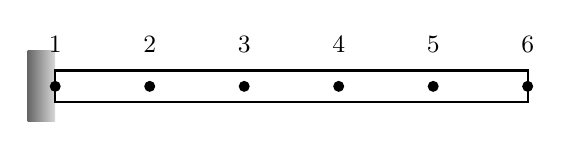
\begin{tikzpicture}[scale=1.0,font=\small]
  \fill[left color=black!60,right color=black!15] (-0.35,-0.45) rectangle (0,0.45);
  \draw[thick] (0,-0.2) rectangle (6,0.2);
  \foreach \i in {1,...,6}{
    \fill ({(\i-1)*1.2},0) circle (0.07);
    \node[above] at ({(\i-1)*1.2},0.3) {\i};}
\end{tikzpicture}

\end{fig}

\topic{Structural level:}
\begin{equation*}
  \Kmat\mat{U} = \Pvec \qquad \text{(obtained by assembling the nodal equilibrium equations)}
\end{equation*}

\section{Compatibility equations}
\topic{Material level}
\begin{enumerate}[label=e.g.\,\arabic*.,leftmargin=*]
  \item $\mat{u}(\mat{x}') = \mat{u}(\mat{x})$ as $\mat{x}'\to\mat{x}$
  \item 2D elasticity problems:
    \begin{equation}
      2\frac{\partial^2\eps_{xy}}{\partial x\,\partial y} = \frac{\partial^2\eps_x}{\partial y^2}+\frac{\partial^2\eps_y}{\partial x^2},
      \qquad\text{where }
      \eps_x = \pd{u}{x},\quad \eps_y=\pd{v}{y},\quad \eps_{xy} = \frac12\Bigl(\pd{u}{y}+\pd{v}{x}\Bigr).
    \end{equation}
    Mathematically, this is called the \emph{integrable condition}. Once this equation is satisfied, we can determine the displacement field from a given strain field.
\end{enumerate}

We all know the integrable condition associated with a conservative force as shown below.
\begin{fig}
  % Work done by a force along a path from point 1 to point 2
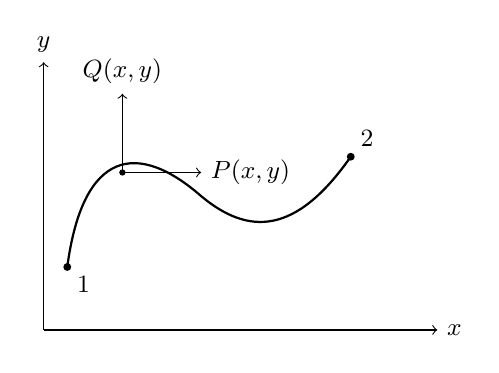
\begin{tikzpicture}[scale=1.0,font=\small]
  \draw[->] (0,0) -- (5.0,0) node[right] {$x$};
  \draw[->] (0,0) -- (0,3.4) node[above] {$y$};
  \draw[thick] (0.3,0.8) .. controls (0.5,2.3) and (1.2,2.4) .. (2.0,1.7)
               .. controls (2.6,1.2) and (3.2,1.2) .. (3.9,2.2);
  \fill (0.3,0.8) circle (0.05) node[below right] {1};
  \fill (3.9,2.2) circle (0.05) node[above right] {2};
  \coordinate (Q) at (1.0,2.0);
  \fill (Q) circle (0.04);
  \draw[->] (Q) -- ++(1.0,0) node[right] {$P(x,y)$};
  \draw[->] (Q) -- ++(0,1.0) node[above] {$Q(x,y)$};
\end{tikzpicture}

\end{fig}
\begin{gather}
  \mat{F} = P(x,y)\,\mat{i} + Q(x,y)\,\mat{j}, \qquad d\mat{r} = dx\,\mat{i} + dy\,\mat{j} \\
  \int_1^2 \mat{F}\cdot d\mat{r} = \int_1^2 P(x,y)\,dx + Q(x,y)\,dy = \int_1^2 dW = -\int_1^2 dV = V_1 - V_2
\end{gather}
Note that the potential energy $V$ exists when $\mat{F}$ is conservative. The work done by a force needs to be evaluated by integration along the path of the particle. However, for a conservative force, no integration is needed. The work done can be evaluated using the change in the potential energy.
\begin{gather}
  \Longrightarrow\quad -dV = -\pd{V}{x}dx - \pd{V}{y}dy = P(x,y)\,dx + Q(x,y)\,dy \\
  \Longrightarrow\quad P(x,y) = -\pd{V}{x},\quad Q(x,y) = -\pd{V}{y}
  \qquad\Longrightarrow\quad \pd{P}{y} = \pd{Q}{x}
\end{gather}

Consider two well-known conservative forces and their potentials.
\begin{enumerate}[label=(\alph*)]
  \item \textbf{Gravity force}
    \begin{fig}
      % Gravity force acting on a particle
\begin{tikzpicture}[scale=1.0,font=\small]
  \draw[->] (0,0) -- (4.5,0) node[right] {$x$};
  \draw[->] (0,0) -- (0,3.2) node[above] {$y$};
  \shade[ball color=black!40] (1.2,1.8) circle (0.22);
  \draw[->] (1.42,1.8) -- ++(0.9,0) node[right] {$P(x,y)$};
  \draw[->] (1.2,2.02) -- ++(0,0.9) node[above] {$Q(x,y)$};
\end{tikzpicture}

    \end{fig}
    \begin{gather*}
      P(x,y) = 0, \qquad Q(x,y) = -mg \\
      \text{Check: } \pd{P}{y} = \pd{Q}{x} \;\Rightarrow\; 0 = 0 \\
      dW = (-mg)\,dy \;\Rightarrow\; dV = -dW = mg\,(dy) \;\Rightarrow\; V = mgy + c
    \end{gather*}
  \item \textbf{Spring (along the $x$-direction) force}
    \begin{gather*}
      P(x,y) = -kx, \qquad Q(x,y) = 0 \\
      \text{Check: } \pd{P}{y} = \pd{Q}{x} \;\Rightarrow\; 0 = 0 \\
      dW = (-kx)\,dx \;\Rightarrow\; dV = -dW = kx\,(dx) \;\Rightarrow\; V = \tfrac12 kx^2 + c
    \end{gather*}
\end{enumerate}

\topic{Nodal level}
E.g.\ for a plane truss, $(u_1,u_2)_1 = (u_1,u_2)_2 = (u_1,u_2)_3$, where a subscript represents the member number.
\begin{fig}
  % Compatibility at a truss node: three members share the same nodal displacements
\begin{tikzpicture}[scale=1.0,font=\small]
  \coordinate (N) at (0,0);
  \draw[member] (N) -- (-1.3,-2.0); \draw[member] (N) -- (0.4,-2.0); \draw[member] (N) -- (1.9,-1.7);
  \fill (N) circle (0.06);
  \draw[->,thick] (N) -- (1.4,0) node[right] {$u_1$};
  \draw[->,thick] (N) -- (0,1.2) node[right] {$u_2$};
  \node[circle,draw,inner sep=1pt] at (-1.1,-0.85) {\scriptsize 1};
  \node[circle,draw,inner sep=1pt] at (-0.2,-1.3) {\scriptsize 2};
  \node[circle,draw,inner sep=1pt] at (1.3,-0.8) {\scriptsize 3};
\end{tikzpicture}

\end{fig}

Skew support: no penetration, i.e.\ the displacement perpendicular to the skew support equals zero.
\begin{fig}
  % Skew (inclined) roller support: no penetration, v = 0
\begin{tikzpicture}[scale=1.0,font=\small,rotate=35]
  % ground surface
  \draw[thick] (-1.6,0) -- (1.8,0);
  \fill[hatch] (-1.6,-0.3) rectangle (1.8,0);
  % roller
  \draw[fill=white] (0,0.3) circle (0.3);
  % attached wedge (member end)
  \draw[thick] (-0.9,0.75) -- (0.6,0.6) -- (-0.5,1.5) -- cycle;
  % tangential displacement u
  \draw[->,thick] (0.4,0.85) -- (1.6,0.85) node[above] {$u$};
  % normal displacement v = 0
  \draw[->,thick] (0.6,-1.3) -- (0.6,-0.35) node[pos=0,below] {$v=0$};
\end{tikzpicture}

\end{fig}

\section{Constitutive equations}
\topic{Material level}
Stress--strain relationships; for linearly elastic material $\bs{\sigma} = \mat{C}\bs{\eps}$ or $\bs{\eps} = \mat{S}\bs{\sigma}$, where $\mat{C} =$ elasticity matrix and $\mat{S} =$ compliance matrix.

\topic{3D problems:}
\begin{equation}
  \mat{C} = \frac{E}{1+\nu}
  \begin{bmatrix}
    \dfrac{1-\nu}{1-2\nu} & \dfrac{\nu}{1-2\nu} & \dfrac{\nu}{1-2\nu} & 0 & 0 & 0\\[8pt]
    \dfrac{\nu}{1-2\nu} & \dfrac{1-\nu}{1-2\nu} & \dfrac{\nu}{1-2\nu} & 0 & 0 & 0\\[8pt]
    \dfrac{\nu}{1-2\nu} & \dfrac{\nu}{1-2\nu} & \dfrac{1-\nu}{1-2\nu} & 0 & 0 & 0\\[8pt]
    0 & 0 & 0 & 1 & 0 & 0\\
    0 & 0 & 0 & 0 & 1 & 0\\
    0 & 0 & 0 & 0 & 0 & 1
  \end{bmatrix}
\end{equation}
\begin{equation}
  \mat{S} = \frac{1}{E}
  \begin{bmatrix}
    1 & -\nu & -\nu & 0 & 0 & 0\\
    -\nu & 1 & -\nu & 0 & 0 & 0\\
    -\nu & -\nu & 1 & 0 & 0 & 0\\
    0 & 0 & 0 & 1+\nu & 0 & 0\\
    0 & 0 & 0 & 0 & 1+\nu & 0\\
    0 & 0 & 0 & 0 & 0 & 1+\nu
  \end{bmatrix}
\end{equation}

\topic{2D problems:}
\begin{description}[style=nextline,leftmargin=1.5em]
  \item[\underline{Case 1: plane stress}]
    Assumption: $\sigma_{zz} = \sigma_{zx} = \sigma_{zy} = 0$ and in-plane ($xy$-plane) loading.
    \begin{fig}
      % Plane stress: thin plate loaded in its own plane
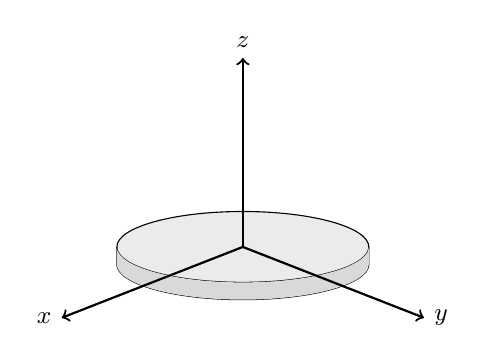
\begin{tikzpicture}[scale=1.0,font=\small]
  % thin disc
  \fill[black!8] (0,0) ellipse (1.6 and 0.45);
  \draw (0,0) ellipse (1.6 and 0.45);
  \draw (-1.6,0) -- (-1.6,-0.22) arc (180:360:1.6 and 0.45) -- (1.6,0);
  \fill[black!15] (-1.6,-0.22) arc (180:360:1.6 and 0.45) -- (1.6,0) arc (360:180:1.6 and 0.45) -- cycle;
  % axes
  \draw[->,thick] (0,0) -- (0,2.4) node[above] {$z$};
  \draw[->,thick] (0,0) -- (-2.3,-0.9) node[left] {$x$};
  \draw[->,thick] (0,0) -- (2.3,-0.9) node[right] {$y$};
\end{tikzpicture}

    \end{fig}
    \begin{equation}
      \mat{C} = \frac{E}{1-\nu^2}\bmat{1 & \nu & 0\\ \nu & 1 & 0\\ 0 & 0 & 1-\nu}, \qquad
      \mat{S} = \frac{1}{E}\bmat{1 & -\nu & 0\\ -\nu & 1 & 0\\ 0 & 0 & 1+\nu}
    \end{equation}
  \item[\underline{Case 2: plane strain}]
    Assumption: $\eps_{zz} = \eps_{zx} = \eps_{zy} = 0$ and in-plane ($xy$-plane) loading.
    \begin{fig}
      % Plane strain: long prismatic body loaded uniformly along its length
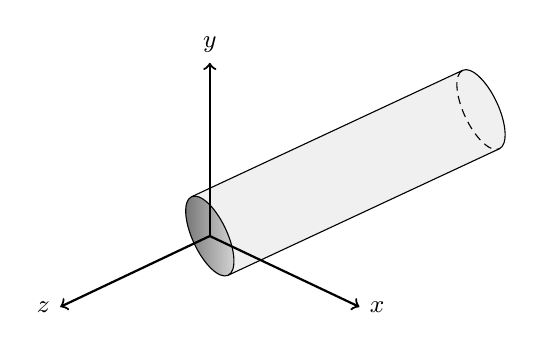
\begin{tikzpicture}[scale=1.0,font=\small]
  % cylinder along a diagonal direction
  \begin{scope}[rotate=25]
    \fill[black!6] (0,-0.55) -- (3.8,-0.55) arc (270:450:0.22 and 0.55) -- (0,0.55) arc (90:270:0.22 and 0.55) -- cycle;
    \draw (0,-0.55) -- (3.8,-0.55); \draw (0,0.55) -- (3.8,0.55);
    \draw (3.8,-0.55) arc (270:450:0.22 and 0.55);
    \draw[densely dashed] (3.8,0.55) arc (90:270:0.22 and 0.55);
    \shade[left color=black!55,right color=black!15] (0,0) ellipse (0.22 and 0.55);
    \draw (0,0) ellipse (0.22 and 0.55);
  \end{scope}
  % axes
  \draw[->,thick] (0,0) -- (0,2.2) node[above] {$y$};
  \draw[->,thick] (0,0) -- (1.9,-0.9) node[right] {$x$};
  \draw[->,thick] (0,0) -- (-1.9,-0.9) node[left] {$z$};
\end{tikzpicture}

    \end{fig}
    \begin{equation}
      \mat{C} = \frac{E}{1+\nu}
      \begin{bmatrix}
        \dfrac{1-\nu}{1-2\nu} & \dfrac{\nu}{1-2\nu} & 0\\[8pt]
        \dfrac{\nu}{1-2\nu} & \dfrac{1-\nu}{1-2\nu} & 0\\[8pt]
        0 & 0 & 1
      \end{bmatrix}, \qquad
      \mat{S} = \frac{1}{E}
      \bmat{1-\nu^2 & -\nu(1+\nu) & 0\\ -\nu(1+\nu) & 1-\nu^2 & 0\\ 0 & 0 & 1+\nu}
    \end{equation}
\end{description}
\noindent$*$ Note that the $\mat{C}$ and $\mat{S}$ matrices for 2D problems can be derived from those for 3D problems using Gauss elimination; we shall do it in class.

\topic{Cross-section level}
Usually called \emph{generalized stress--strain relationships}, e.g.\ axial force--axial strain relationship ($F = EA\eps$), moment--curvature relationship ($M = EI\phi$), and torsion--rate of twist relationship ($T = GJ\theta'$).
